\documentclass[twocolumn]{ctexart}
\usepackage{ctex}
\usepackage{amsmath}

%首行缩进两字符 利用\indent \noindent进行控制
\usepackage{indentfirst}
\setlength{\parindent}{2em}

%算法包
\usepackage{caption}
\usepackage{algorithm}
\usepackage{algorithmic}

%页边距包
\usepackage{geometry}
\geometry {left=2.0cm ,right=2.0cm,top=2.5cm,bottom=2.5cm}

%枚举
\usepackage{enumerate}

%算法input output
\renewcommand{\algorithmicrequire}{\textbf{Input:}} % Use Input in the format of Algorithm
\renewcommand{\algorithmicensure}{\textbf{Output:}} % Use Output in the format of Algorithm

%数学符号
\usepackage{amssymb}
\usepackage{wasysym}
%图片
\usepackage{graphicx}

%表格
\usepackage{booktabs}
\usepackage{multirow}

%Tikz画图
\usepackage{tikz}
\usetikzlibrary{arrows,graphs} %指明是图库
\usetikzlibrary{positioning,automata}

%\usegdlibrary
\begin {document}
	\title{Problem Set 5 Answer Sheet}
	\author{\textbf{151220131谢旻晖}}
	\date{}
	\maketitle
	
\section*{Problem 6.1}
\indent $n-2$

\section*{Problem 6.2}
\noindent 1.\\
\indent 第一个点是我们手动设定的,无需比较。\\
\indent
从第二个点开始,每次$getMin$将第$i$个节点加入$tree$,要对所有$fringe$的点中比较以得最小权者($n-i$次cmp),同时需要对所有其他的$fringe$点进行$updateFringe$($n-i$次cmp)。\\
\[
	\sum_{i=2}^{n}n-i+n-i=(n-1)(n-2)
\]
\\
\noindent 2.\\
\indent $n-1$

\section*{Problem 6.5}
\noindent 1.\\
\indent 将图所有边权取负,求新图的MST,再将所有边权恢复,MST即为最大权重生成树。\\
\noindent 2.\\
\indent 求最大权重生成树的补图,其中所有的边形成的集合为最小的反馈边集。

\section*{Problem 6.6}
\indent 是不可能的。下面证明:最短路径树与任何最小生成树都至少共用一条边。\\
\indent 证明:考虑从$s$点开始,我们使用$Prim$算法构造MST的过程,第一步,我们从所有与$s$相连的边中选出权最小的那条边(设为$s\rightarrow v$),此时我们就保证了$s$到$v$的最短路径是$s\rightarrow v$,换而言之,$s\rightarrow v$一定既在MST中,又在SSSPT中。证毕。

\section*{Problem 6.7}
\noindent\textbf{case a:}仍然不变\\
\textbf{case b:}把修改的边加入原生成树,在生成的环中去掉权值最大的边(破圈)\\
\textbf{case c:}仍然不变\\
\textbf{case d:}将修改的边删除,原生成树形成两个连通分量,可以用SCC算法识别出两个连通分量,接着遍历所有的边,找到其中权值最小的且连接两个连通分量的边,加入。\\


\section*{Problem 6.8}
\indent 令$\varPhi=V-U$,$\varPsi=\{(x,y)|x,y\in\varPhi \wedge (x,y)\in E\}$,首先考虑图$G'=(\varPhi,\varPsi)$的MST,如果$G'$都不连通,则最轻生成树显然不存在,如果连通,我们求出$G'$的最小生成树$T$。\\
\indent 接着考虑边集$\Gamma=\{(x,y)|x\in\varPhi \wedge y\in U \wedge (x,y)\in E \}$
,不断选$\Gamma$中权值最小的边加入$T$,以将$U$中的结点连接至$T$,已连接过的结点不再重复连接。直到将$U$中的结点全部连接完毕,$T$为最轻生成树。若$U$中有点与$T$不连通,则不存在最轻生成树。

\section*{Problem 6.9}
\indent $Krystal$改进版本:设G的边集为E,首先将S中的所有边选入,然后在E-S中不断选不与已选边构成环且权值最小的边,直到总共选满$|G.V|-1$条边。

\section*{Problem 6.11}
\noindent 命题正确。\\
\indent $\Rightarrow$\\
\indent 采用反证法,如果$T$是$G$的MST,但$T$不是$G'$的MST。那么$G'$一定存在一个权值比$T$小的最小生成树$T'$。根据平方关系,$T'$在$G$中的权也小于$T$,与$T$是$G$的MST矛盾,假设不成立。所以$T$是$G$的最小生成树,那$T$一定也是$G'$的最小生成树。\\

\indent $\Leftarrow$\\
\indent 同理。

\section*{Problem 6.12}
\noindent1.\\
\indent 若不为唯一,则至少存在一条边


\section*{Problem 6.13}
\noindent1.\\
\indent 易证,有用边一定是割边,

\section*{Problem 6.14}
\noindent 容易举出一个反例\\
\begin{center}
	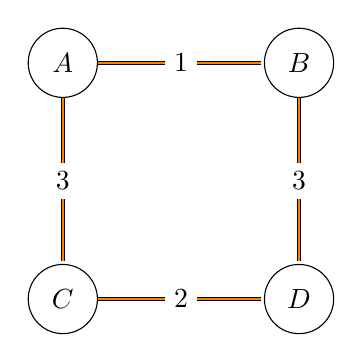
\begin{tikzpicture}[>=stealth',shorten >=1pt,node distance=3cm,on grid,initial/.style    ={}]
	\node[state]          (A)                        {$A$};
	\node[state]          (B) [right =of A]    {$B$};
	\node[state]          (C) [below =of A]    {$C$};
	\node[state]          (D) [below =of B]    {$D$};
	\tikzset{every node/.style={fill=white}} 
	\tikzset{mystyle/.style={-,double=orange}}   
	\path
	(A)     edge [mystyle]   node   {$1$} (B)
	(A)     edge [mystyle]   node   {$3$} (C) 
	(C)     edge [mystyle]   node   {$2$} (D)
	(B)     edge [mystyle]   node   {$3$} (D);
	
%	\draw [dashed] (1.5,1.3)--(1.5,-3);
	
	\end{tikzpicture}
\end{center}


%\begin{figure}[!h]
%	\centering
%	\includegraphics[width=0.2\textwidth]{6.13.png}
%\end{figure}
\indent 如图所示,令$V_1=\{A,C\}$,$V_2=\{B,D\}$,利用题意中的分治算法求出的MST为\{AB,AC,BD\},权为7,而实际上的最小生成树为\{AB,CD,AC\}或\{AB,CD,BD\},权为6。

\section*{Problem 6.15}
\indent 首先,如果一个生成树是第二小的生成树,那么他一定与某棵最小生成树仅有一边之差。然后,先用$Kruskals$算法求出原图的MST,接着我们尝试删去MST中的每条边,在此基础上再次运行$Kruskals$算法构建生成树(注意不能用删去的边),计算此树与MST的权差,找到其中权差最小但\textbf{非0}(避免找到MST)的ST,即为次小生成树。\\


\section*{Problem 6.16}
在此图上运行$Dijkstra$算法,源点为S,会错误地得到S->B的最短路径为2的结论。
\begin{center}
	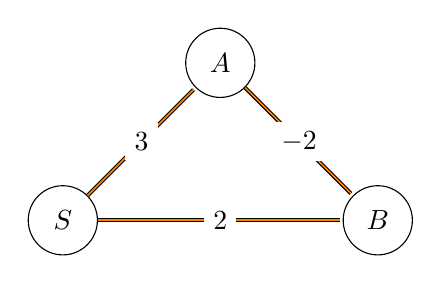
\begin{tikzpicture}[>=stealth',shorten >=1pt,node distance=3cm,on grid,initial/.style    ={}]
	\tikzset{every node/.style={circle}}
	\node[state] (A) at (0,0)        {$S$};
	\node[state] (B) at (2,2)        {$A$};
	\node[state] (C) at (4,0)        {$B$};
	\tikzset{every node/.style={fill=white}} 
	\tikzset{mystyle/.style={-,double=orange}}   
	\path
	(A)     edge [mystyle]   node   {$3$} (B)
	(A)     edge [mystyle]   node   {$2$} (C) 
	(B)     edge [mystyle]   node   {$-2$} (C);
	
	\end{tikzpicture}
\end{center}
\indent$Dijkstra$由于是贪心的,每次都找一个距源点最近的点(dmin),然后将该距离定为这个点到源点的最短路径(d[i]<--dmin);但如果存在负权边,那就有可能先通过并不是距源点最近的一个次优点,再通过这个负权边生成的路径之和更小。

\section*{Problem 6.17}
\indent 给定源点为S,在下图中生成的最短路径树为\{SA,SB\},但MST为\{SB,BA\}。
\begin{center}
	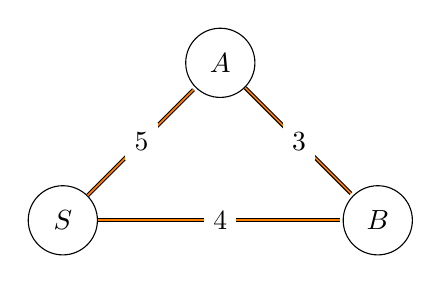
\begin{tikzpicture}[>=stealth',shorten >=1pt,node distance=3cm,on grid,initial/.style    ={}]
	\tikzset{every node/.style={circle}}
	\node[state] (A) at (0,0)        {$S$};
	\node[state] (B) at (2,2)        {$A$};
	\node[state] (C) at (4,0)        {$B$};
	\tikzset{every node/.style={fill=white}} 
	\tikzset{mystyle/.style={-,double=orange}}   
	\path
	(A)     edge [mystyle]   node   {$5$} (B)
	(A)     edge [mystyle]   node   {$4$} (C) 
	(B)     edge [mystyle]   node   {$3$} (C);
	
	\end{tikzpicture}
\end{center}

\end {document}
